\documentclass{beamer}

% choose theme (warning, to use the UniBern theme you need to copy the files beamerthemeUniBern.sty and ublogo.pdf in the same directory)
\usetheme{UniBern}

% packages
\usepackage{hyperref} % allows clickable urls
\usepackage{dsfont} % allow ds font

% define title page
\title{\LaTeX \ for scientists }
\subtitle{ }
\author{Julien Riou}
\date{13 February 2019}
\institute{institute}

% begin document
\begin{document}

\frame{\titlepage}

\frame{
	\frametitle{Plan}
	\begin{itemize}
		\item What is \LaTeX ?
		\item Writing and compiling \LaTeX \ code
		\item Basic formatting
		\item Advanced topics
		\item \LaTeX \ templates for scientists:
			\begin{itemize}
				\item[-] cover letter  
				\item[-] scholarly article
				\item[-] journal submission
				\item[-] presentation
			\end{itemize}

	\end{itemize}


}


\frame{
	\frametitle{\LaTeX \ is \ldots}
	
	\ldots a sophisticated \alert{typesetting system}.
	
	\medskip\pause
	
	Different from a ``\textit{what you see is what you get}" word processor:
	\begin{itemize}
		\item \alert{program} the structure and contents of a document
		\item compile the \LaTeX \ code into an output file (PDF)
	\end{itemize}

	\medskip\pause
	
	Very good for:
	\begin{itemize}
		\item professional-looking documents with a \alert{pre-specified format}
		\item structure, reproductibility
		\item maths, cross-referencing, bibliographies
	\end{itemize}

	\medskip\pause
	
	Less good for:
	\begin{itemize}
		\item creating highly personalized documents
	\end{itemize}
	
}


\frame{
	\frametitle{Writing and compiling \LaTeX \ code}
	\textit{In principle}, you only need a text editor and a \LaTeX \ compiler:
	\begin{itemize}
		\item write your code and save it as a \texttt{.tex} file
		\begin{itemize}
			\item[-] e.g. with notepad in Windows
		\end{itemize}
		\item compile the \texttt{.tex} file into an output file (generally  \texttt{.pdf})
		\begin{itemize}
			\item[-] e.g. with MiK\TeX \ for Windows or \TeX \ Live for MacOS and Linux
		\end{itemize}
	\end{itemize}		
	\bigskip\pause
	
	\textit{In practice}, it is easier to use an integrated development environment:
		\begin{itemize}
			\item installed on your computer: \alert{\TeX Studio} (\url{www.texstudio.org}) 
				\begin{itemize}
					\item[-] but you still need to install a compiler!
				\end{itemize}		
			\item online: \alert{Overleaf} (\url{www.overleaf.com})
		\end{itemize}
}


\frame{
	\frametitle{Commands}
	\LaTeX~ commands start with \alert{\textbackslash} and are of two kinds:
	\begin{block}{Declarations}
		\begin{itemize}
			\item Are stated once and take effect until further notice
		\end{itemize}
		e.g. \texttt{\textbackslash documentclass}, \texttt{\textbackslash centering},  \texttt{\textbackslash textit\{\}}
	\end{block}
	\begin{block}{Environments}
		\begin{itemize}
			\item Have matching \texttt{begin} and \texttt{end} declarations
		\end{itemize}
		e.g. \texttt{\textbackslash begin\{itemize\} \ldots \textbackslash end\{itemize\}} 
	\end{block}
	\medskip
	\alert{Beware}, forgetting closing braces or end declarations will give an error!
}


\frame{
	\frametitle{Arguments}
	\begin{block}{Required arguments\ldots}
		\begin{itemize}
			\item Are contained in curly braces
			\item Must be included
		\end{itemize}
		e.g. \texttt{\textbackslash documentclass\{\underline{letter}\}}
	\end{block}
	\begin{block}{Optional arguments\ldots}
		\begin{itemize}
			\item Are contained in square brackets
			\item Can be left out
			\item Give you more control over the commands
		\end{itemize}
		e.g. \texttt{\textbackslash documentclass[\underline{12pt}]\{letter\}}
	\end{block}
}

\frame{
	\frametitle{A basic \texttt{.tex} file}
	\begin{enumerate}
		\item Declare the type of document you want (\texttt{book, article, letter, report}\ldots) with  \texttt{\textbackslash documentclass} \vspace{.5em}

		\item Declare additional options or packages (\texttt{float, amsmath, geometry}\ldots) with  \texttt{\textbackslash usepackage} \vspace{.5em}

		\item Write your content within a \texttt{document} environment \vspace{1em} \pause
		
		\hspace{1em}\texttt{\textbackslash documentclass\{\}} \\
		\hspace{1em}\texttt{\%\textbackslash usepackage\{\}} \\
		\hspace{1em}\texttt{\textbackslash begin\{document\}} \\
		\hspace{2em}\ldots\\
		\hspace{1em}\texttt{\textbackslash end\{document\}}
	\end{enumerate}

}
%
%\frame{
%	\frametitle{Document class}
%	\LaTeX~has several basic templates selected using \texttt{\textbackslash documentclass}:
%	\begin{itemize}
%		\item book, article, report, letter \ldots
%	\end{itemize}
%	
%	\pause
%	\begin{block}{Options:}
%		\begin{itemize}
%			\item Default font size: \texttt{10pt}, \texttt{11pt}, \texttt{12pt}
%			\item Paper size: \texttt{a4paper}, \texttt{letterpaper}
%			\item Printing: \texttt{twoside}, \texttt{oneside}
%		\end{itemize}
%	\end{block}
%	For example, if you want a report to be in 12pt type on A4, but printed one-sided, you would use:\vspace{.3em}
%	
%	\hspace{1em}\texttt{\textbackslash documentclass[12pt,a4paper,oneside]\{report\}}
%	
%}




\frame{
	\frametitle{Hello, world!}
	Let's try a simple ``Hello, world!'' example with \LaTeX~and Overleaf:
	\begin{itemize}
		
		\item Go to \url{www.overleaf.com} and log in with your credentials
		
		\item Create a new project, then an empty document named \texttt{helloworld.tex} 
		
		\item Create a \texttt{letter} that says ``Hello, world!'' \pause
		
		\begin{block}{Solution}
			\vspace{.3em}
			\hspace{5em}\texttt{\textbackslash documentclass\{letter\}} \\
			\hspace{5em}\texttt{\%\textbackslash usepackage\{\}} \\
			\hspace{5em}\texttt{\textbackslash begin\{document\}} \\
			\hspace{8em}Hello, world! \\
			\hspace{5em}\texttt{\textbackslash end\{document\}}
	\end{block}
	\end{itemize}
}

\frame{
	\frametitle{Basic formatting}
	\begin{itemize}
		\item font styles
		\item special characters
		\item lists
		\item sectioning
		\item figures
		\item cross-referencing
		\item bibliography
		\item equations
	\end{itemize}
}

\frame{
	\frametitle{Font style}
\begin{block}{Font face:}
	\texttt{\textbackslash textit\{}\textit{Text}\texttt{\}},
	\texttt{\textbackslash textbf\{}\textbf{Text}\texttt{\}}, 
	\texttt{\textbackslash texttt\{}\texttt{Text}\texttt{\}}, 
	\texttt{\textbackslash textsc\{}\textsc{Text}\texttt{\}} \ldots
\end{block}\pause
\begin{block}{Font size:}
	\texttt{\textbackslash tiny\{\tiny{Text}}\texttt{\}},
	\texttt{\textbackslash scriptsize\{\scriptsize{Text}}\texttt{\}},
	\texttt{\textbackslash footnotesize\{\footnotesize{Text}}\texttt{\}},
	\texttt{\textbackslash small\{\small{Text}}\texttt{\}},
	\texttt{\textbackslash large\{\large{Text}}\texttt{\}},
	\texttt{\textbackslash Large\{\Large{Text}}\texttt{\}},
	\texttt{\textbackslash huge\{\huge{Text}}\texttt{\}}
\end{block}\pause
\begin{block}{Alignment:}
	\texttt{\textbackslash begin\{center/flushright/flushleft\}\\
		\ldots\\
		\textbackslash end\{center/flushright/flushleft\}}
\end{block}
}

\frame{
	\frametitle{Special characters and commands}
			\begin{block}{Special commands}
		\texttt{\textbackslash} or $\sim$ $\rightarrow$ extra single space \\
		\texttt{\textbackslash \textbackslash} $\rightarrow$ new line \\
		\texttt{\textbackslash hspace\{1cm\}} or \texttt{\textbackslash vspace\{5mm\}} $\rightarrow$ custom space \\
		\texttt{\textbackslash clearpage} $\rightarrow$ new page \\
	\end{block}	\pause
		\begin{block}{Non-standard characters:}

		 \texttt{\textbackslash \%} $\rightarrow$ \% (used for commenting out)\\
		 \texttt{\textbackslash \&} $\rightarrow$ \& (used for separations) \\
		 \texttt{\textbackslash \{} $\rightarrow$ \{ (used in commands) \\
		 \texttt{\textbackslash textbackslash} $\rightarrow$ \textbackslash \ (used in commands) \\ \vspace{.2cm}
		 \textit{and lots of other symbols:} $\spadesuit$, $\phi$, $\mathfrak{R}$, $\mathcal{R}$, $\dagger$, $\lll$, $\notin$, $\triangle$\ldots (try \texttt{detexify})  \\
		\end{block}

		
}

\frame{
	\frametitle{Lists}
	\begin{block}{Bullet list:}
		\vspace{2mm}
		\begin{columns}
			\column{0.6\textwidth}
			\hspace{1.5cm}\texttt{\textbackslash begin\{itemize\} \\
				\hspace{2cm}\text\textbackslash item} Text \\
			\hspace{2cm}\texttt{\textbackslash item}[-] Text \\
			\hspace{1.5cm}\texttt{\textbackslash end\{itemize\}}
			\column{0.4\textwidth}
			\begin{itemize}
				\item Text
				\item[-] Text
			\end{itemize}
		\end{columns}
	\end{block}\pause
	\begin{block}{Numbered list:}
		\vspace{2mm}
		\begin{columns}
			\column{0.6\textwidth}
			\hspace{1.5cm}\texttt{\textbackslash begin\{enumerate\} \\
				\hspace{2cm}\text\textbackslash item} Text \\
			\hspace{2cm}\texttt{\textbackslash item} Text \\
			\hspace{1.5cm}\texttt{\textbackslash end\{enumerate\}}
			\column{0.4\textwidth}
			\begin{enumerate}
				\item Text
				\item Text
			\end{enumerate}
		\end{columns}
	\end{block}\pause
\vspace{1em}
Note: Lists can be nested within other lists.
}

\frame{
	\frametitle{Sectioning}
	\LaTeX~ can \alert{organize, number, and index} sections of document: \\\vspace{.5em}
	
	\hspace{1em}\texttt{\textbackslash section\{Introduction\}}\vspace{.7em} \hspace{3em}{\large \textbf{1 Introduction}}
	
	\hspace{1em}\texttt{\textbackslash subsection\{Context\}}\vspace{.7em} \hspace{4.5em}\textbf{1.1 Context}
		\pause
		
	\begin{block}{Layers of sectioning}
	
		\hspace{2mm} \textcolor{gray}{\large{ \textbackslash part\{\}}   
		\textbackslash chapter\{\} }
		{\small \textbackslash section\{\}}  
		{\footnotesize  \textbackslash subsection\{\}}  
		{\scriptsize \textbackslash subsubsection\{\}}
		{\tiny \textbackslash paragraph\{\}}
	\end{block}
	\vspace{1em}\pause
	For the unnumbered version, add an asterisk: \\\vspace{.5em}
	
	\hspace{1em}\texttt{\textbackslash section*\{Introduction\}} \hspace{3em}{\large \textbf{ Introduction}} \pause
	
	\vspace{1.5em}Note: Add a table of contents with \texttt{\textbackslash tableofcontents}
}

\frame{
	\frametitle{Figures}
	Figures must be added as \alert{independent files} in the same repertory. \\\vspace{.3em}	\pause
		\texttt{\hspace{1cm}\textbackslash begin\{figure\}[h] \\
				\hspace{1.5cm}\textbackslash centering \\
				\hspace{1.5cm}\textbackslash includegraphics[width=2cm,height=3cm]\{cat.png\} \\
				\hspace{1.5cm}\textbackslash caption\{This is my cat.\} \\				
				\hspace{1cm}\textbackslash end\{figure\}}\pause
	\begin{block}{Placement options:}
		\vspace{-3mm}
		\begin{itemize}
			\item \texttt{h}: 	approximately at the same point it occurs in the code
			\item \texttt{t}/\texttt{b}: 	at the top/bottom of the page
			\item \texttt{p}: 	on a special page for figures only
			\item \texttt{H}: 	\textit{precisely} at the same point in the code (requires a package: \texttt{\textbackslash usepackage\{float\}})
		\end{itemize}
	\end{block}
}

\frame{
	\frametitle{Cross-referencing}
	\LaTeX \ handles all references using \alert{unique identifiers}.
		\begin{itemize}
			\item place a label after something (section, figure caption...) \\
	\texttt{
		\hspace{.7cm}\textcolor{gray}{\textbackslash begin\{figure\}[ht]} \\
		\hspace{1.5cm}\textcolor{gray}{\textbackslash centering} \\
		\hspace{1.5cm}\textcolor{gray}{\textbackslash includegraphics\{cat.png\}} \\
		\hspace{1.5cm}\textcolor{gray}{\textbackslash caption\{This is my cat.\}} \\
		\hspace{1.5cm}\textbackslash label\{\textcolor{blue}{refcat}\} \\				
		\hspace{1cm}\textcolor{gray}{\textbackslash end\{figure\}}
	}\vspace{.5em}\pause
			\item then refer to the same identifier at any point in the text \\\vspace{.5em}
			
				 \hspace{1cm}\texttt{My cat is very cute (see Fig.\textbackslash ref\{\textcolor{blue}{refcat}\}}).\\\vspace{.3em}
				 
				  \hspace{2cm}$\rightarrow$ My cat is very cute (see Fig. 1).
		\end{itemize}
}

\frame{
	\frametitle{Bibliography I}
	Same principle for citing books or articles, except that the information must be placed in a \alert{separate bib\TeX~file} in the same repertory.
	\begin{itemize}
		\item use the \texttt{\textbackslash cite} command instead:\vspace{.3em}
		
		\hspace{-.9cm}\texttt{My cat is the product of evolution\textbackslash cite\{\textcolor{blue}{darwin1859origin}\}}. \vspace{.3em}\pause
		
		\item place the corresponding information in a separate \texttt{foo.bib} file:\\\vspace{.3em} 
		
		\texttt{
			\hspace{.7cm}@book\{\textcolor{blue}{darwin1859origin}, \\
				\hspace{1.5cm}title=\{On the origin of species\},\\
				\hspace{1.5cm}author=\{Darwin, Charles\},\\
				\hspace{1.5cm}year=\{1859\} \}
		}
		\vspace{.3em}\pause
		\item add a reference to the \texttt{foo.bib} file at the end of the source file:\\\vspace{.3em}
		
		\texttt{
			\hspace{.7cm}\textbackslash bibliographystyle\{plain\} \\
			\hspace{.9cm}\textbackslash bibliography\{foo\}	
	}
	\end{itemize}
}

\frame{
	\frametitle{Bibliography II}
	Several basic \alert{styles} are included (\texttt{apalike, unsrt, abbrv}) and journal-specific styles can be added. \\\vspace{2em}
	
	The bib\TeX~ file can be created:
	\begin{itemize}
		\item manually 
		\item copied from e.g. \url{https://scholar.google.ch/}
		\begin{figure}[h]
			\centering
			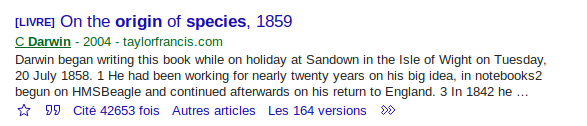
\includegraphics[height=2cm]{google_scholar.png}
		\end{figure}
		
		\item directly from Zotero or Endnote (export as bibtex)
	\end{itemize}
}


\frame{
	\frametitle{Equations I}
	\LaTeX~allows you to typeset any sort of equations with \alert{reliability}.
	\begin{block}{Using math mode}
		Inline math mode: \texttt{\$\ldots\$}
		\begin{center}
			Consider subject $i \in \{1,\ldots,n\}$...
		\end{center}
		
		Numbered equations: 		\texttt{\small \textbackslash begin\{equation\}\ldots\textbackslash end\{equation\}}
		\begin{equation}
			 \text{logit} \ \mathds{E}(Y) = \alpha+\beta x
		\end{equation}
	\end{block}
}

\frame{
	\frametitle{Equations II}
	Some commands:
\begin{center}
	\begin{tabular}{rl}
		$4+2$ & \texttt{\$4+2\$} \\ \pause
		$\sqrt{5}$ & \texttt{\$\textbackslash sqrt\{5\}\$} \\ \pause
		$\frac{x}{y}$ & \texttt{\$\textbackslash frac\{x\}\{y\}\$} \\ \pause
		$Y^{m}_{i}$ & \texttt{\$Y\^{}\{m\}\_\{i\}\$} \\ \pause
		$\sum_{i=1}^n x_i$ & \texttt{\$\textbackslash sum\_\{i=1\}\^{}n x\_i\$} \\ \pause
		$Y \sim \mathcal{N}(0,1)$ & \texttt{\$Y \textbackslash sim \textbackslash mathcal\{N\}(0,1) \$} \\ \pause
		$\alpha \in \{\alpha,\beta\}$ & \texttt{\$\textbackslash alpha \textbackslash in \textbackslash \{\textbackslash alpha,\textbackslash beta\}\$} \\ \pause
		$f''(\xi)$ & \texttt{\$f''(\textbackslash xi)\$} \\ \pause
		180$^{\circ}$C & \texttt{180\$\^{}\{\textbackslash circ\}\$C} \\
	\end{tabular}

\end{center}
}

\frame{
	\frametitle{Advanced topics}
	\framesubtitle{Tables I}
	Creating tables manually can be \alert{tricky}. \\\vspace{1em}

	\begin{columns}
		\column{0.7\textwidth}
			\texttt{	
				\textbackslash begin\{table\}[h] \\
				\hspace{.5cm}\textbackslash centering \\
				\hspace{.3cm} \only<2->{\textbackslash begin\{tabular\}\{\textcolor{blue}{r|c|c}\} } \\
				\hspace{.8cm}  \only<3->{Trial \& n \& t \textbackslash\textbackslash~\textbackslash hline} \\
				\hspace{.8cm}  \only<4->{1 \& 23 \& 2 \textbackslash\textbackslash~\textbackslash hline} \\
				\hspace{.8cm}  \only<5->{2 \& 15 \& 10 \textbackslash\textbackslash~\textbackslash hline} \\
				\hspace{.8cm}  \only<6->{3 \& 100 \& 20 \textbackslash\textbackslash~} \\
				\hspace{.3cm}  \only<2->{\textbackslash end\{tabular\}} \\
				\hspace{.2cm}\textbackslash end\{table\}
			}
		\column{0.3\textwidth}
		\begin{table}
			\centering
			\begin{tabular}{r|c|c} 
				Trial & n & t \\ \hline
				1 & 23 & 2 \\ \hline
				2 & 15 & 10 \\ \hline
				3 & 100 & 20 \\ 
			\end{tabular}
		\end{table}
	\end{columns}
	\vspace{-3em}
}

\frame{
	\frametitle{Advanced topics}
	\framesubtitle{Tables II}
	Beyond simple tables it is preferable to use \alert{dedicated tools}:
	\begin{itemize}
		\item online convertors (e.g. \url{https://tablesgenerator.com/})
		\item R package: \texttt{xtable}
		\item Stata function: \texttt{esttab}
	\end{itemize}
}



\frame{
	\frametitle{Advanced topics}
	\framesubtitle{Collaborating}
	From simple to more difficult (but more powerful):
	\begin{itemize}
		\item drafting in Word and pasting the final version into \LaTeX \pause
		\item using comments in the source code \\
			\texttt{\hspace{1em}\% this sentence is really stupid}\pause
		\item inline additions in the compiled PDF  \\
			\texttt{\hspace{1em}\textbackslash textcolor\{red\}\{SAD!\}}\pause
		\item writing in margins (or in boxes with package \texttt{\alert{todonotes}})\\
			\texttt{\hspace{1em}\textbackslash marginpar\{you are fired\}}\pause
		\item highlighting modifications using \texttt{\alert{latexdiff}} \pause
		\item version control: paid overleaf account, \texttt{svn}, \texttt{\alert{git}}
	\end{itemize}
	\vspace{-1cm}
}

\frame{
	\frametitle{\LaTeX \ templates for scientists}

	Templates to fill the needs of scientists:
	\begin{itemize}
		\item \alert{scholarly article}
		\item journal submission
		\item letters (cover letter, answer to reviewers)
		\item presentation
	\end{itemize}
	
	\vspace{1em}
	Download the files from: \\
	\centering\underline{\smash{\url{https://github.com/jriou/LaTeX_for_scientists}}}
}


\frame{
	\frametitle{\LaTeX \ templates for scientists}
	\framesubtitle{Scholarly article}
	Creating \alert{professional-looking} articles with the same methods used by journal publishers.
	\vspace{1em}
	
	Very important for \alert{directly published} academic documents:
	\begin{itemize}
		\item preprints (e.g. for bioRxiv)
		\item supplementary appendices
	\end{itemize}\pause

	\begin{block}{How to use it}
	\begin{itemize}
		\item upload all 3 files in \texttt{/scholarly\_article} to Overleaf
		\item select \texttt{scholarly\_article.tex} and hit the ``recompile'' button
	\end{itemize}
\end{block}
\vspace{-2.5em}
}

\frame{
	\frametitle{\LaTeX \ templates for scientists}
	\framesubtitle{Journal submission}
	Some academic journals provide \LaTeX~templates for submissions (e.g., PLoS Medicine \href{https://journals.plos.org/plosmedicine/s/latex}{\underline{here}}). \pause
	
	\begin{block}{How to use it}
		\begin{itemize}
			\item upload all 2 files in \texttt{/plos\_submission\_template} to Overleaf
			\item select \texttt{plos\_latex\_template.tex} and hit the ``recompile'' button
		\end{itemize}
	\end{block}
}



\frame{
	\frametitle{\LaTeX \ templates for scientists}
	\framesubtitle{Letters}
	Provided by the University  (\href{http://intern.unibe.ch/dienstleistungen/corporate_design_und_vorlagen/index_ger.html}{\underline{here}})\\\vspace{.3em}
	
	Especially useful for \alert{cover letters} and \alert{responses to reviewers} \pause
	
	\begin{block}{How to use it}
		\begin{itemize}
		\item open the \texttt{/cover\_letter} repertory
		\item open the \texttt{.clo} file in any editor to modify the personal settings
		\item comment out the 5th line (starting with ``\texttt{\textbackslash PackageError}'')
		\item upload all 5 files to Overleaf
		\item start your letter from the \texttt{.tex} file
		\begin{itemize}
			\item[-] options in \textbackslash \texttt{documentclass[]}: english/german, color/bw...
			\item[-] recipient address, subject, opening, main text, closing
		\end{itemize}
	\end{itemize}
	\end{block}
	\vspace{-1.3cm}
}

\frame{
	\frametitle{\LaTeX \ templates for scientists}
	\framesubtitle{Presentation}
	\alert{Surprise} (?) this presentation was made in \LaTeX! \\\vspace{.5em}
	
	There is a document class called \texttt{\alert{beamer}} that allows to do presentations (a template is provided by the University \href{http://intern.unibe.ch/dienstleistungen/corporate_design_und_vorlagen/praesentationen/index_ger.html}{\underline{here}}).\\\vspace{.3em} \pause
	
	\begin{block}{How to use it}
		\begin{itemize}
			\item upload all 4 files in \texttt{/beamer} to Overleaf
			\item select \texttt{unibern-demo.tex} and hit the ``recompile'' button
		\end{itemize}
	\end{block}
}

\frame{
	\frametitle{Acknowledgments}
	\begin{itemize}
		\item 	MIT Introduction to \LaTeX~(\underline{\href{https://web.mit.edu/rsi/www/pdfs/new-latex.pdf}{link}})
		\item 	Peter Flom, \LaTeX~for academics and researchers who (think they) don't need it. (\underline{\href{https://www.tug.org/TUGboat/tb28-1/tb88flom.pdf}{link}})
		\item \LaTeX~wikibook (\underline{\href{https://en.wikibooks.org/wiki/LaTeX}{link}})
		\item \LaTeX~cheat sheet (\underline{\href{http://wch.github.io/latexsheet/}{Winston Chang}}) 
	\end{itemize}

	

}


\end{document}
